\documentclass[12pt,letterpaper]{article}
\usepackage[T1]{fontenc}
\usepackage[utf8]{inputenc}  % Accents codés dans la fonte
\usepackage[french]{babel}   % Les traductions françaises
\usepackage{numprint}        % \numprint(9,36) pour utilisation de la virgule comme séparateur décimal
\usepackage{amsmath}         % Les maths de base
\usepackage[svgnames]{xcolor}% Pour les besoins de PythonTeX
\usepackage{geometry}        % Gestion des dimensions des pages
\usepackage{tgpagella}       % Pour changer un peu les fontes
\usepackage{tgadventor}
\usepackage{inconsolata}
\usepackage{booktabs}        % Beaux tableaux avec \toprule, etc.
\usepackage{multirow}        % Fusionner des cellules d'un tableau
\usepackage{multicol}
\usepackage{graphicx}        % Gestion des inclusions graphiques
\usepackage{siunitx}        % Gestion des inclusions graphiques
\DeclareSIUnit\angstrom{\text {Å}}
\usepackage{graphicx}
\graphicspath{ {Figures/} }
\usepackage{tikz}            % Si on veut présenter le code Python
\usepackage[framemethod=TikZ]{mdframed}
\usepackage{csquotes}
\usepackage{enumitem}

\usepackage[backend=biber,style=nature,intitle=true]{biblatex}
\addbibresource{./tp.bib}
\DefineBibliographyStrings{french}{in={,},inseries={}}

% Un environnement pour faire joli pour présenter le code Python
\newenvironment{code}{%
\begin{mdframed}[linecolor=Green,innerrightmargin=30pt,innerleftmargin=30pt,
backgroundcolor=Black!5,
skipabove=10pt,skipbelow=10pt,roundcorner=5pt,
splitbottomskip=6pt,splittopskip=12pt]
}{%
\end{mdframed}
}

% Présentation de l'abstract pour la problématique
\usepackage[runin]{abstract}

% Un environnement pour la problématique
\newenvironment{problematique}{
\renewcommand{\abstractname}{But}
\begin{abstract}
}{
\end{abstract}
}

% Titre et auteurs du document
\title{TP CPH409 - Liaison chimique, aspect statique}
\author{Alexandre Fleury}
\date{XX juillet 2022}

% Et début du document proprement dit
\begin{document}
\renewcommand{\labelitemi}{$\bullet$}
\maketitle

\begin{problematique}
Nous appliquerons, lors de ce travail pratique, différents modèles sur les électrons $\pi$ de l'anion du cyclopentadiène. Nous comparerons les modèles de la particule confinée dans un cercle, le modèle de Hückel et les calculs numériques du package PySCF.
\end{problematique}

\section*{Votre mission, que vous accepterez}
Vous modéliserez et analyserer des calculs sur le système $\pi$ de l'anion du cyclopentadiène.
\begin{center}
  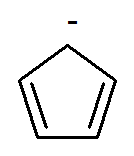
\includegraphics[width=.1\linewidth]{clyclopentadiene_anion.png}
\end{center}

Pour ce faire, vous aurez accès à une approximation de la fonction d'onde électronique de cette molécule calculée à l'aide de PySCF, un répertoire de codes en python pour la chimie quantique. Comme vous avez appris en cours, lorsque vous aurez la fonction d'onde $\psi$, vous pourez extraire les propriétés du système. Vous allez calculer les valeurs propres  d'énergie des orbitales, les coefficients associés et visualiser leur apparence. Ensuite, vous comparerez les orbitales (énergies, dégénérescence) obtenus à l'aide des différents modèles de la particule confinée dans un cercle et de Hückel.

\section*{Modèles simples}
\subsection*{Particule confinée dans un cercle}

En considérant le problème de la particule dans un cercle
\begin{equation}
-\frac{\hbar^2}{2m} \left( \frac{\partial^2}{\partial x^2} + \frac{\partial^2}{\partial y^2} \right) \psi = E \psi
\end{equation}

Nous pouvons simplifier le problème en utilisant les coordonnées polaires ($r$ et $\phi$).
\begin{align}
\label{Hxy} \hat{H} &= -\frac{\hbar^2}{2m} \left( \frac{\partial^2}{\partial x^2} + \frac{\partial^2}{\partial y^2} \right) \\
\label{Hrphi} &= -\frac{\hbar^2}{2m} \left( \frac{\partial^2}{\partial r^2} + \frac{1}{r} \frac{\partial}{\partial r} +  \frac{1}{r^2} \frac{\partial^2}{\partial \phi^2} \right) \\
&= -\frac{\hbar^2}{2mr^2} \frac{d^2}{d \phi^2} = -\frac{\hbar^2}{2I} \frac{d^2}{d \phi^2}\quad\text{(}r\text{ constant)}
\end{align}

En considérant que le confinement dans un cercle implique que $\psi(\phi) = \psi(\phi + 2\pi)$, les solutions peuvent être exprimées ainsi
\begin{equation}
\Phi = A e^{i m_l \phi} + B e^{-i m_l \phi}
\end{equation}

Et les énergies associées comme
\begin{equation}
E_{m_l} = \frac{m_l^2 \hbar^2}{2I}\quad\text{où}\ m_l=0,\pm 1,\pm 2, ...
\label{vpropre}
\end{equation}

Où $\hbar$ et $I$ sont respectivement la constante de planck divisé par $2\pi$ et le moment d'inertie $m r^2$.
\begin{enumerate}
\item Porter en schéma (versus un axe d'énergie) les orbitales $m_l=0,\pm 1, \pm 2$. Considérer la masse de l'électron à \SI{9.109e-31}{\kilo\gram} et fixer le diamètre du cercle à \SI{2.276}{\angstrom}.
\item Placer les électrons du système $\pi$ de l'anion du cyclopentadiène sur ce schéma.
\item Démontrer que les valeurs propres de la particule confinée dans un cercle sont égales à l'équation~(\ref{vpropre}).
\item Démontrer que l'équation (\ref{Hxy}) est égale à~(\ref{Hrphi}).
\end{enumerate}


\subsection*{Modèle de Hückel}

Nous avons vu en cours le modèle de Hückel dans la partie 11.
\begin{enumerate}[resume]
\item Écrire la matrice du déterminant séculaire pour l'anion du cyclopentadiène.
\item Résoudre le déterminant.
\item Porter en schéma les énergies des orbitales en fonction de $\alpha$ et $\beta$. Considérer que $\beta=\SI{-75}{\kilo\joule\per\mole}$ \cite{mcquarrie}.
\item Placer les électrons du système $\pi$ de l'anion du cyclopentadiène dans le schéma.
\item Trouver les coefficients de l'orbitale moléculaire de plus basse énergie, en considérant
\begin{align}
\psi_{min} &= \sum^{5}_{i=1} c_i \cdot p_{zi} \\
1 &= \sum^{5}_{i=1} c_i c_i^*
\end{align}
où $\psi_{min}$, $c_i$ et $p_{zi}$ sont respectivement la fonction d'onde de l'orbitale moléculaire d'énergie minimale, le coeffcient de l'atome $i$ et l'orbitale $2p_z$ de l'atome $i$. 
\item Discuter de la validité de ce dessin pour l'orbitale de plus basse énergie.
\begin{center}
\end{center}
\end{enumerate}

\section*{Calculs numériques}

Normalement, la résolution numérique de l'équation de Schrödinger pour des molécules nécessitent l'installation de logiciel ou la construction d'un environnement de travail. Un des ces environnements de travail est le Jupyter Notebook, qui permet de coder tout en conservant les variables créées et de produire des graphiques. Vous travaillerez dans un notebook hébergé sur Google colab, ce qui permet de faire les calculs nécessaires dans un fureteur internet sans rien installer localement sur votre ordinateur. Pour accéder aux notebooks:

\begin{description}
\item[Tutoriel] \url{https://colab.research.google.com/github/alexfleury/cph409/blob/main/notebooks/Chimie_quantique.ipynb}
\item[Espace de travail] \url{https://colab.research.google.com/github/alexfleury/cph409/blob/main/notebooks/TP.ipynb}
\end{description}

\begin{enumerate}[resume]
\item Compléter le tableau suivant pour montrer l'effet de l'ajout d'orbitales.
\begin{center}
  \begin{tabular}{cccc}
      \toprule
      Ensemble de base & \# orbitales supplémentaires & Énergie & Temps de calcul \\
      \midrule
      3-21G & 0 & & \\
      6-31G & 0 & & \\
      6-31G(d,p) &  & & \\
      6-31G(2d,2p) &  & & \\
      6-31G(3d,3p) &  & & \\
      6-31G(3df,3pd) &  & & \\
      \bottomrule
  \end{tabular}
\end{center}

\item Même chose que précédemment, pour montrer l'effet du nombre de $\zeta$ dans l'ensemble de bases.
\begin{center}
  \begin{tabular}{cccc}
    \toprule
    Ensemble de base & \# de $\zeta$ & Énergie & Temps de calcul \\
    \midrule
    STO-3g &  & & \\
    6-31G & & & \\
    6-311G &  & & \\
    \bottomrule
  \end{tabular}
\end{center}

\item Quelle est la différence en énergie avec le calcul avec les bases 6-31G(d,p) et 6-31+G(d,p)? Le «+» fait référence à l'ajout de fonctions diffuses, qui s'étendent plus loin dans l'espace que les fonctions gaussiennes. Pourquoi l'ajout du «+» est nécessaire pour bien décrire la densité électronique des anions?
\item Faire un ou des graphique(s) de l'énergie en fonction du \# d'orbitales supplémentaires et du \# de $\zeta$.
\item Discuter des résultats en lien avec la méthode variationnelle.
\item Identifier l'orbitale liante de moindre énergie du systèmes $\pi$ dans le calcul fait avec l'ensemble de base STO-3G. Faire un schéma (axe d'énergie) des orbitales HOMO-2 jusqu'à LUMO+1 et placer les électrons.
\item Extraire les coefficients de l'orbitale HOMO-2.
\end{enumerate}

\section*{Questions}
\begin{enumerate}[resume]
\item Comparer les schémas des orbitales (vs un axe d'énergie) obtenues grâce aux 3 méthodes. En considérant la valeur publiée de 5.14 eV pour le gap HOMO-LUMO~\cite{doi:10.1021/om00036a047}, discuter des résultats (différences d'énergie HOMO-LUMO, dégénérescence, orbitales frontières, ...).
\item Discuter brièvement des forces/faiblesses des modèles que nous avons abordés.
\item Comparer les coefficients des orbitales obtenues avec la méthode Hartree-Fock et avec la méthode de Hückel.
\item Décriver comment feriez-vous pour savoir quelle méthode de calcul quantique (méthode de calcul, choix de l'ensemble de base, code/programme à utiliser, etc.) est la plus appropriée pour un problème donné? Discuter.
\end{enumerate}

\section*{Rapport}
\subsection*{Remise}
La remise est juste avant l'examen final.
\subsection*{Format}
Mettre seulement les choses demandées à chaque section (ne pas faire un rapport classique de chimie). Vous pouvez faire les schémas et les démonstrations à la main (stylo) si vous le souhaitez.

\nocite{*}
\printbibliography[]

\end{document}
